\chapter{绪论}
\section{研究的背景和意义}
%这是测试\cite{seugs:standard}

车辆的行驶是由驾驶人操纵有关机构实现的,驾驶人不仅是道路交通系统的信息处理者和决策者,也是道路交通系统的调节者和控制者,是道路交通系统中最活跃的要素。车辆的行驶状态是驾驶人所采取的驾驶行为的作用结果,而驾驶行为是在一定的外部环境下,驾驶人生理、心理和操作技能等驾驶特性相互作用的综合体现。不同驾驶人的生理状况和心理素质不同、驾驶操作技能也有差异,因此驾驶行为存在差异。不同驾驶人表现出不同的驾驶行为,同一名驾驶人在不同的外部环境和自身状态下的驾驶行为也不同。驾驶人行为特性具体的外在表现主要包括,在动态交通条件下,驾驶人的反应时间,速度选择,加速度选择,跟驰距离选择,变道决策与间隙接受等一系列特性。

长期以来,我国机动车为各种企事业单位所有,机动车驾驶人均为专业驾驶人,专业驾驶人的驾驶技能熟练程度、驾驶特性等方面的差异都较小。随着大量小汽车进入家庭,产生了大量的非专业驾驶人,非专业驾驶人在生理、心理以及驾驶操作技能等方面与专业驾驶人都存在明显的差异。而在传统的道路交通规划、设计与交通管理的研究和工程设计中,从宏观上假设驾驶人的驾驶特性相似和受同一普遍规律影响。这种假设没有体现驾驶人操作活动在复杂环境下的不确定性和不一致性,没有反映同一驾驶人在不同环境下驾驶行为特性的差异,没有反映大量驾驶人驾驶特性的微观差异对宏观交通流的影响,没有反映出驾驶人不同的驾驶特性对道路交通流的影响作用关系,这与现今真实的交通状况存在显著的差异。在此基础上进行的道路交通规划、设计与交通管理难以符合真实的交通现象,降低了交通规划、设计方案与交通管理措施的合理性与实施效果,同时也增加了交通事故的潜在危险性。

通过研究驾驶人行为特性对交通流的影响,将有助于对驾驶特性、驾驶行为与道路交通流的影响关系有更加深刻的理解;将有助于从人的因素的角度分析各种复杂交通流现象的形成和演化过程;将有助于确定影响道路交通安全的人的因素,为进一步探究改善交通流状况和提高交通安全性提供有力的理论支持;也可以为智能车辆、驾驶辅助支持系统等设备的研制提供理论支持。总之,研究驾驶人行为特性对道路交通流的影响,对提高道路交通系统运输效率和交通安全性具有重要意义,对我国今后的道路交通规划、设计、管理、控制也有重要的理论和应用价值。



\section{国内外研究概况}
与本文议题相关的国内外相关研究主要集中在三个方面,1)驾驶人行为特性研究,2)驾驶人与驾驶行为建模,3)驾驶人行为与交通流关系研究。

\subsection{驾驶人行为特性研究}
对驾驶人行为特性研究可以分为两种思路,一种主要考察了不同道路条件下的驾驶人行为特性,另一种则考察了不同属性驾驶人的行为特性,这些研究主要通过实际观测的手段对驾驶人的行为特性进行了比较和分析,为理解驾驶人的行为特性提供了经验基础。

\subsubsection{不同道路条件下的驾驶人行为特性}
对不同道路条件下的驾驶人行为特性的研究,主要针对某一特定的道路条件下的驾驶人行为进行了分析。Kou(1997)研究了高速公路汇入匝道处驾驶人的跟驰和汇入时的间隙接受行为。研究发现驾驶人匝道处的汇入行为,并不与任何单一的参数如汇入速度、主线流量、跟车间距与时距、速度差等显著相关,而各参数的组合能更好的解释驾驶人的驾驶行为\cite{Kou1997}。Heaslip(2007)在跟驰模型中加入了驾驶人对车道改变的熟悉程度、适应性和驾驶人的进攻性,研究了施工区域驾驶人的驾驶行为\cite{Heaslip2007}。Xu(2007)研究了环形交叉口驾驶人的间隙接受行为,研究从视频数据中提取事件信息,用最大似然法和Raff法对临界车头时距和跟车时距进行了估计并进行了比较。研究发现交织流量和环道车速与临界车头时距和跟车时距呈现负相关性\cite{Xu2007}。Dalia Said(2008)根据高速公路不同路段的实测数据,从驾驶人劳动强度的角度分析了驾驶人的加减速和方向盘操作行为,并与高速公路线形设计的安全性进行了关联性分析\cite{Said2008}。

\subsubsection{不同属性驾驶人的行为特性}
不同属性驾驶人的行为特性的研究,通过对不同性别、驾驶经验等属性的驾驶人行为的观测,比较分析了不同驾驶人行为的差异性。孔繁森 (2004) 依据Kuipers的定性仿真方法对熟练驾驶人和刚学会开车的驾驶人,在具有不同曲率半径和路面情况的一段道路上所做出的车速选择做了定性推理,给出了两类不同驾驶人驾车行为的定性状态描绘图和相应的车速曲线变化图\cite{孔繁森2004}。Yang(2007)通过对加拿大城市道路、乡村道路和高速公路的实测数据对自由流和非自由条件下的驾驶人的速度选择和加减速行为进行了研究,并对不同行为的驾驶人进行了分类。研究发现对于不同的道路驾驶人的速度行为差异明显,并与交通流条件高度相关;驾驶人一般会选择高于限速值不超过10\%的速度;根据驾驶人群体可分为进攻型、防守型、和一般型三类,进攻型倾向于选择高于限速的车速,防守型相反,一般型选择不超过限速太多的车速;驾驶人的加减速选择在非自由流条件下变化更大;在自由流条件下,驾驶人的加减速依赖于瞬时速度。在中低速情况下,加减速率随速度增加而减小。而在高速条件下较为稳定;不同类型驾驶人的加减速选择差异明显,进攻型驾驶人加减速率较大而防守型相反\cite{Yang2008}。张开冉 (2008) 对新驾驶人的反应时间进行测试,与一定样本量的对照组相应指标作比较,结果表明信息复杂度较大时,两组间反应时差异较为显著\cite{张开冉2008}。王晶 (2008) 基于驾驶人性别对城市快速路跟驰模型进行了研究\cite{王晶2008}。徐上(2009)在实际道路交通环境下进行了驾驶人跟驰行为实验,测试了驾驶人的跟驰距离、跟驰时距等操作特征参数。研究发现:性别因素、驾驶人精神状态因素、驾龄和累计行驶里程对跟驰时距有较为显著的影响;男性驾驶人跟驰时距较女性驾驶人平均低约 0.7s;驾龄和累计行驶里程越长,跟驰时距相应越小,但并非是线性减少关系\cite{徐上2009}。

\subsection{驾驶行为建模}
对驾驶行为建模主要可分为微观交通流模型和基于驾驶人认知与决策的模型。微观交通流模型主要从交通流理论中的基本图出发,通过对车辆相对位置关系和运动的描述对驾驶人行为建模。而基于驾驶人认知与决策的模型,对驾驶过程中的复杂的认知和决策行为进行了研究。
\subsubsection{微观交通流模型}
微观交通流模型将驾驶行为分为跟驰和变道两种行为,主要有影响力的跟驰模型包括GM模型,期望参数模型,优化速度模型,Gipps模型,IDM模型等。各模型所假设驾驶人的跟驰目的不尽相同,但均主要围绕速度差,跟驰距离等变量建立模型。

变道模型一般将变道分为强制变道和非强制变道,变道行为分为两个阶段,车道选择和间隙接受。具体的跟驰模型和变道模型将在第二章展开描述。

目前的微观交通流模型将跟驰和变道单独研究,认为两者相互独立,而这并不符合实际,Toledo 等(2007)提出了一个整合加速、车道变换、间隙接受等各种驾驶行为模型的框架,研究了驾驶人变道过程中的加速行为\cite{Toledo2007}。


\subsubsection{基于驾驶人认知与决策的模型}
随着对驾驶人行为研究的深入,越来越多的研究对驾驶人的认知、决策等活动进行了考虑,并将其纳入到驾驶人的建模当中。Oliver和Pentland(2000)在测试车数据基础上利用组对隐马尔科夫模型对驾驶人行为进行了识别和预测\cite{Oliver2000}。邱凌云 (2005) 基于Agent理论对驾驶人进行建模.研究了Agent的跟驰、换道和挤占道等行为\cite{邱凌云2005}。Dario D.Salvucci(2006)基于ACT-R的认知模型对驾驶人的转向操作、跟驰、变道准备和变道行为、注视分布进行了研究\cite{Salvucci2006}。杨新月 (2006) 基于认知活动链对驾驶人行为进行了建模和仿真\cite{杨新月2006}。许骏 (2008) 将驾驶人-汽车看作统一的人机系统,建立了基于Markov决策过程的驾驶人行为模型,并对所建模型进行了计算机仿真\cite{许骏2008}。王晓原 (2008) 基于决策树对驾驶行为决策机制进行了研究\cite{王晓原2008}。Samer Hani Hamdar(2009)对驾驶人行为进行建模,把驾驶行为作为一种随机的冒险行为进行研究,从而将人的认知过程纳入到微观交通流模型中,并且发现驾驶人预期、驾驶人行为差异和驾驶经验长短对其行为有显著影响\cite{Hamdar2009a}。

由于考虑驾驶人认知决策的模型的复杂性,这些模型还需要更多的证据来证明其有效性和优越性。


\subsection{驾驶人行为与交通流关系研究}
由于驾驶人的行为特性很难大范围调查,研究驾驶人行为与交通流关系,目前主要使用基于模型模拟的方法。而所研究的主要驾驶行为特性是驾驶人的跟驰行为特性。

雷丽等(2003)在一维交通流元胞自动机NaSch模型的基础上,优先考虑驾驶员的不确定性敏感预期行为,将随机延迟过程放在确定性减速之前,从而建立一种新的一维元胞自动机交通流模型,研究发现敏感驾驶因素对车流的作用很大,随着敏感驾驶车辆的增多,道路容量随之提高\cite{雷丽2003}。葛红霞等(2005)研究发现当考虑快车和慢车的混合交通流时,即使少量的慢车也会导致交通流量大幅度下降\cite{葛红霞2005}。李启朗 (2006) 在单车道元胞自动机交通流NS模型基础上,通过引入不同的刹车概率来反映不同驾驶人的驾驶特性,并在周期边界条件下,对由激进驾驶车辆和谨慎驾驶车辆构成的混合交通流进行模拟.结果表明,在有谨慎驾驶车辆构成的交通流的临界密度以前,混合交通流的流量完全由谨慎驾驶人的特性决定\cite{李启朗2006}。Farzaneh和Rakha(2006)分析了商用的交通流模拟软件中的稳态跟驰模型,并将跟驰模型分为两类,一类假设驾驶人的期望速度不随流量变化,另一类驾驶人的期望速度随流量变化即INTEGRATION中使用的Van Aerde跟驰模型。Farzaneh和Rakha对驾驶人假设不同的期望速度,研究了速度变化对于稳态交通流的影响,发现速度变化对于通行能力所对应的最佳车速有显著的影响\cite{Farzaneh2006}。ZHU等(2007)建立了一个包括不同驾驶人概率的元胞自动机模型,分析了不同驾驶人混合对交通流的影响\cite{H.B.ZHU2007}。Zhu和Dai(2008)研究发现当驾驶人检测车头距的反应延误增加时,交通流稳定区域减小,驾驶人检测车头距的反应延误在交通拥堵转换中扮演重要的角色\cite{Zhu2008}。Ossen(2008)区分并研究了驾驶人之间差异和驾驶人内部差异对交通流的影响,研究发现驾驶人之间差异对基本图的形状产生影响,而驾驶人自身行为差异导致密度-速度平面上在水平轴上散落,导致基本图不再是一条线而成为一个平面。其研究还表明驾驶人的差异程度影响车队的稳定,差异程度低的车队会放大引导车的动态变化,而差异程度高的车队则会平滑引导车的动态变化。并且引导车的动态变化如何传播海域车队组成的顺序有关。而驾驶人的差异性对交通流稳定性的影响与对车队的结果类似\cite{Ossen2008}。祝会兵(2008)研究发现:当道路上有一些比较谨慎的司机时,随机减速概率就大,道路流量明显下降;没有事故车瓶颈和其它瓶颈,慢车对交通流特性有很大的影响;司机的敏感性越差,反应延迟时间越长,越容易产生交通阻塞\cite{祝会兵2008}。Hamdar(2009)对驾驶人行为进行建模,把驾驶行为作为一种随机的冒险行为进行研究,通过模拟实验发现器模型中影响密度-流量基本图的三个主要参数是对碰撞的权重,速度的不确定参数和驾驶人最大的提前预计时间,其他的影响因素还有驾驶人群体是否存在差异,以及驾驶人的反应时间。模拟实验发现驾驶人群体的差异性增加了基本图上点的分散程度,表明驾驶人差异性增加了交通流的不稳定性。而反应时间的增加造成了基本图上点的分散程度的增加和震得下移,意味着反应时间的增加造成了通行能力的下降和交通流的不稳定性\cite{Hamdar2009a}。Kesting等(2010)使用IDM跟驰模型通过模拟研究了,ACC控制车辆的比例对与通行能力的影响,结果表明每增加1\%的ACC车辆,通行能力增加0.3\%\cite{Kesting2010}。

\subsection{国内外研究总结}

目前国内外关于驾驶人行为对交通流影响的研究已取得不少成果,但是还主要存在两点问题。其一,目前使用基于模型模拟的方法研究驾驶行为特性对交通流的影响,主要通过改变模型中的参数或使用不同参数模型进行混合,而所假设改变的参数在实际中是否会出现所假设的变化,目前还没有充分地研究。其二,目前所研究对交通流的影响还主要局限在交通流的效率性方面,较少涉及交通流的安全性。


%国内外针对驾驶人行为的研究集中在驾驶人的认知行为和操作行为上,对认知行为的研究主要包括驾驶人眼动特性,速度、距离等感知特性,驾驶人注意分配特性,驾驶人生理数据的采集分析等。对驾驶人操作行为的研究主要包括驾驶人的一般与特定道路条件下的跟驰行为,换道行为、超车行为等。在现有的研究中,对驾驶人行为差异性的研究基本都是在静态条件下进行比较,缺乏对实际道路交通环境下,车辆动态行驶过程中驾驶人决策和行为的差异性的研究。
%
%国内外针对驾驶人与驾驶行为的建模,逐渐从机械的力学模型发展到控制理论模型,再到跟驰模型和变道模型以及两者相结合的综合模型,在交通流模型中越来越多地考虑到了驾驶人的主观因素,现今已有一些研究考虑了驾驶人的认知和决策过程,有的模型中考虑了驾驶人根据对周围车辆动态的预计和判断对车辆进行操控这一特性,使得驾驶人模型更为符合实际。
%
%国内外对驾驶人与交通流关系的研究主要从两个方面开展,一方面,从微观的角度,通过实际数据的测量以及使用基于驾驶人特性的微观模型进行仿真,通过调整驾驶人行为特性参数来研究驾驶人特性对交通流的影响。另一方面,从宏观交通流模型修正的角度,通过对宏观模型中驾驶人因素项的改进来解释交通流中的幽灵拥堵、相位变化等交通流现象。%两方面的研究均取得了一些成果,但是微观的驾驶人模型与宏观交通流模型之间似乎缺少某种联系,有关研究表明,这种联系可能会存在于驾驶人之间的相互作用之中。

\section{研究内容和论文框架}

\subsection{论文依托}

本论文依托于国家自然科学基金项目:“驾驶人员驾驶特性对道路交通流的影响机理”(50708019)。


\subsection{研究思路和技术路线图}
针对本文的研究背景,在假设驾驶经验对驾驶人行为有影响的前提下,并且在现有研究的基础上,通过对实际观测数据的分析研究,挖掘驾驶人行为特性的差异。通过交通流的微观模拟研究驾驶人行为特性对交通流效率性和安全性的影响。

本文技术路线图如\autoref{tech-path}。

\begin{figure}[htpb]
	\centering
	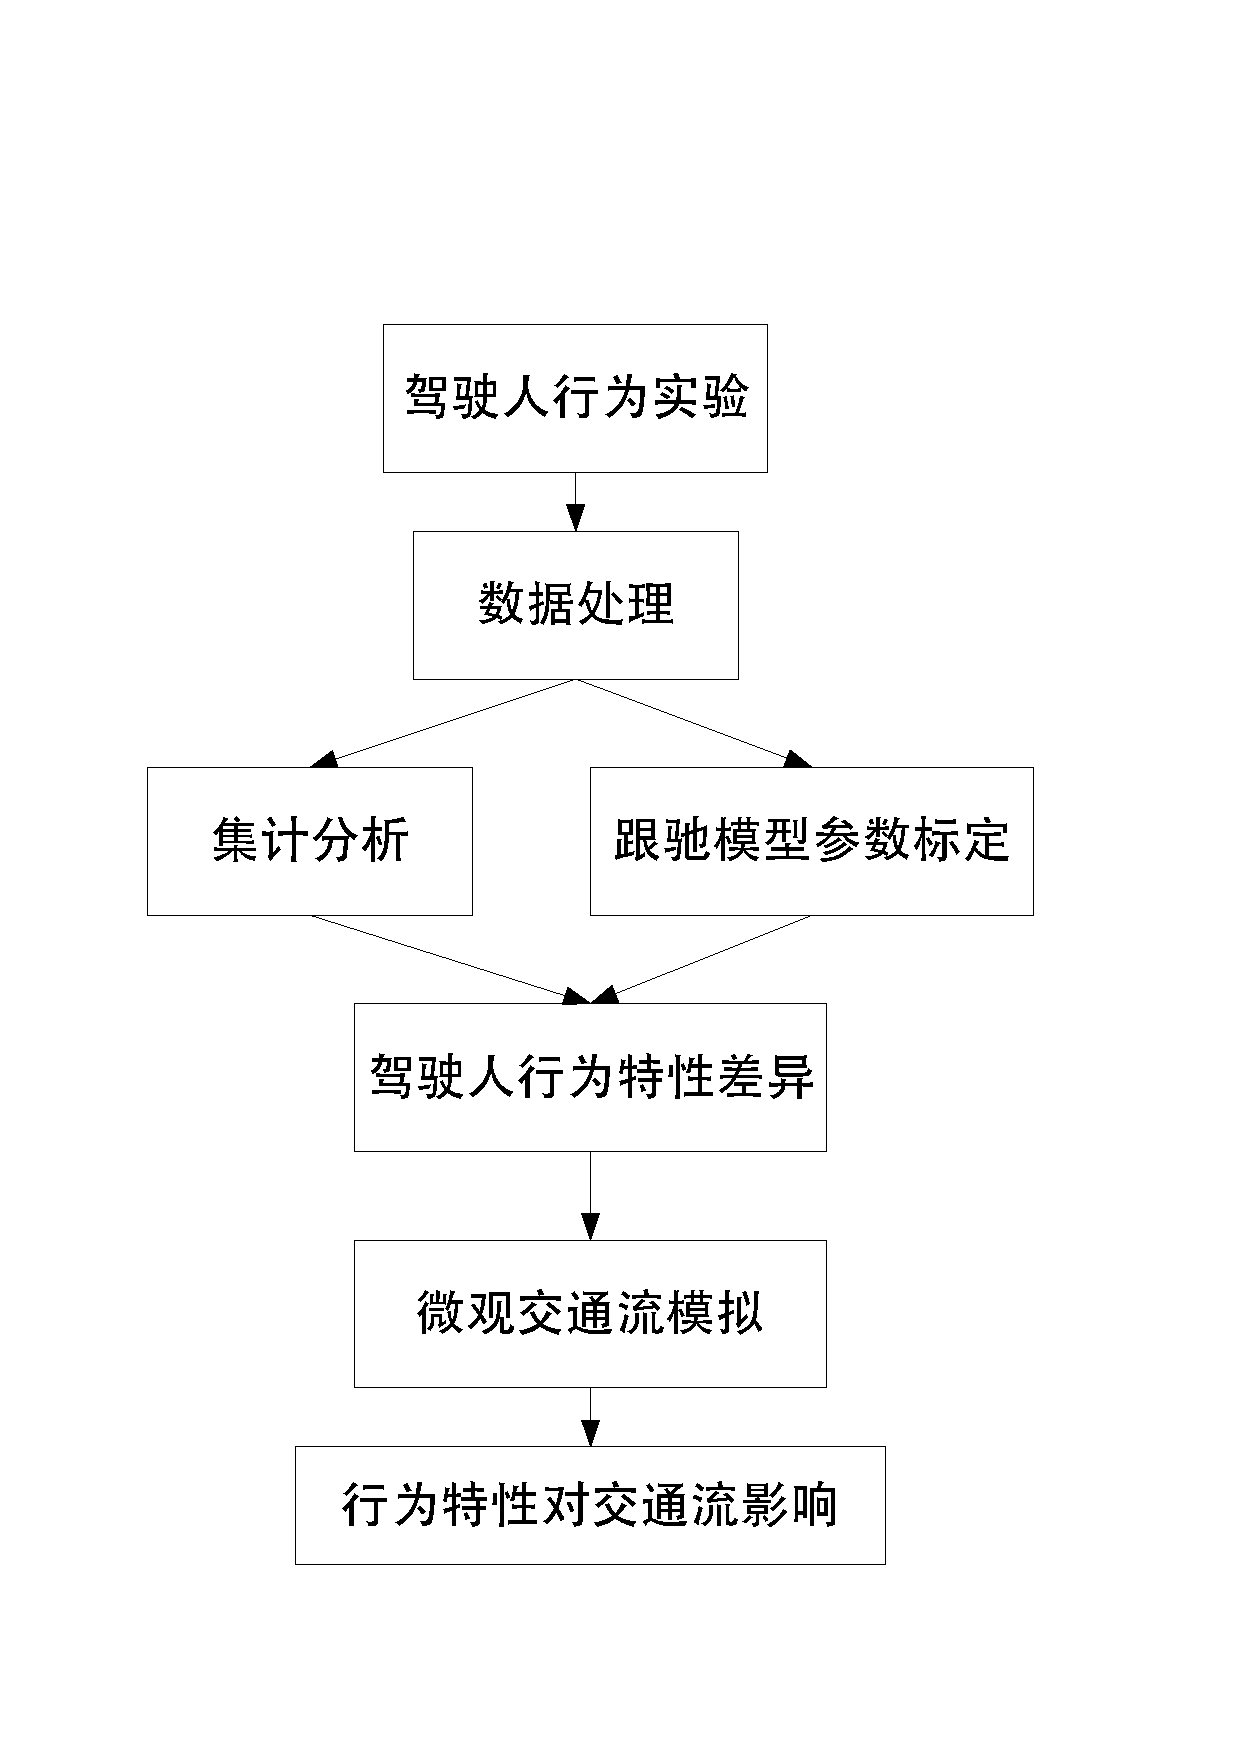
\includegraphics[width=0.4\linewidth]{tech-path}
	\caption{技术路线图}
	\label{tech-path}
\end{figure}

\subsection{研究内容}
根据研究思路,本文的主要研究内容如下:

(1)驾驶人驾驶行为特性主要参数和交通流参数采集

针对本文研究背景,基于驾驶经验对驾驶行为产生影响的假设,以专业和非专业驾驶人为研究对象,调查其性别、年龄、驾龄、行驶里程等基本信息。选择典型的城市道路路段,在良好天气条件下,采集实际交通流状态下驾驶人的跟车速度、跟车间距、加速度、等驾驶行为的主要参数。

(2)驾驶人行为特性分析

根据实验所得的测试车轨迹数据与其邻近车辆的相对速度和相对位置的时间序列数据,分析驾驶人在其动态变化的驾驶环境中的速度选择,加速度选择,跟驰距离选择等特性。通过对数据的集计分析以及跟驰模型的参数标定,分析并比较驾驶过程中的不同驾驶人行为的异同。

(3)驾驶人行为特性对交通流影响分析

应用交通仿真程序,针对不同情况分别进行模拟研究:通过对驾驶人模型参数以及不同类型驾驶人混合比例的调整,研究驾驶人行为特性微观差异对于路段交通流宏观的效率和安全特性的影响。


\section{论文框架}
本文共分六章,本文的组织框架如下:

第一章,绪论,首先论述本文的选题背景及意义,然后介绍国内外关于驾驶行为特性及其对交通流影响的研究现状,接着介绍本文的研究思路,最后介绍本文的主要研究内容。

第二章,驾驶人行为特性及其对交通流影响的含义,阐述本文的研究对象和范围,介绍了表征驾驶人行为特性以及交通流状态的参数和主要有影响力的跟驰和变道模型,论述了驾驶人行为特性差异性的含义。

第三章,驾驶人行为特性实验,介绍了本文数据来源所使用的实验方法和实验过程。

第四章,驾驶人行为特性的差异性分析,通过对实验所获取数据的处理,通过集计分析和跟驰模型的参数标定,分析驾驶人行为特性的差异性。

第五章,驾驶人行为特性对交通流影响分析,使用微观交通流模拟软件,针对不同影响因素进行模拟仿真,分析并阐述阐述驾驶人行为特性对交通流效率性和安全性参数的影响以及可能的解释。

第六章,结论和展望,总结本文主要结论和存在问题,指出今后进一步研究的方向。
%\begin{table}[htbp]
% \centering
% \caption{Add caption}
% \begin{tabular}{cccc}
%   \addlinespace
%    \toprule
%    Face database & Yale  & Caltech & ORL \\
%    \midrule
%    Number of training & \multicolumn{ 1}{c}{5} & \multicolumn{ 1}{c}{3} & \multicolumn{ 1}{c}{3} \\
%    samples per class  & \multicolumn{ 1}{c}{} & \multicolumn{ 1}{c}{} & \multicolumn{ 1}{c}{} \\
%    \bottomrule
%    \end{tabular}
%  \label{tab:addlabel}
%\end{table}
\section{本章小结}

本章叙述了论文研究的背景和意义,总结了国内外驾驶人行为特性及其对交通流影响相关研究的已有成果和不足,提出了本研究的主要内容与技术路线。